\documentclass[12pt,a4paper]{article}
\usepackage[dvipsnames]{xcolor}
\usepackage[utf8]{inputenc}
\usepackage{amsmath}
\usepackage{mathtools}
\usepackage{marvosym}
\usepackage{wrapfig}
\usepackage{hyperref}
\usepackage{float}
\usepackage{multicol}
\hypersetup{colorlinks,citecolor=black,filecolor=black,linkcolor=black,urlcolor=black}
\usepackage{pdfpages}
\usepackage{amsfonts}
\usepackage{amssymb}
\usepackage{fancyhdr}
\usepackage{chemfig}
\usepackage{graphicx}
\usepackage[T1]{fontenc}
\usepackage[magyar]{babel}
\usepackage{bm}
\usepackage{tikz, tcolorbox}
\usetikzlibrary{positioning}
\usepackage{verbatim}
\usepackage{amsmath,esint}
\usepackage{setspace}
\usepackage{qtree}
\usepackage{multido}
\usepackage{mathptmx} % Times New Roman betűtípus
\usepackage{listings}
\usepackage{caption}
\captionsetup[lstlisting]{labelformat=empty}

\lstset{
    language=Matlab,
    inputencoding=utf8,
    extendedchars=true,
    basicstyle=\ttfamily\small,
    frame=single,
    breaklines=true,
    numbers=left,
    numberstyle=\tiny,
    literate=
        {á}{{\'a}}1
        {é}{{\'e}}1
        {í}{{\'i}}1
        {ó}{{\'o}}1
        {ö}{{\"o}}1
        {ő}{{\H{o}}}1
        {ú}{{\'u}}1
        {ü}{{\"u}}1
        {ű}{{\H{u}}}1
        {Á}{{\'A}}1
        {É}{{\'E}}1
        {Í}{{\'I}}1
        {Ó}{{\'O}}1
        {Ö}{{\"O}}1
        {Ő}{{\H{O}}}1
        {Ú}{{\'U}}1
        {Ü}{{\"U}}1
        {Ű}{{\H{U}}}1
}
\renewcommand{\figureautorefname}{ábra}
\newcommand{\abrara}[1]{\hyperref[#1]{\ref*{#1}.~ábra}}
\newcommand{\Pointilles}[1]{%
\par\nobreak
\noindent\rule{0pt}{1.5\baselineskip}% Provides a larger gap between the
\multido{}{#1}{\noindent\makebox[\linewidth]{\dotfill}\endgraf}
\bigskip% Gap between dots and next paragraph
}
\newcommand{\feladat}[1]{%
\phantomsection
\subsection*{#1. feladat}%
\addcontentsline{toc}{subsection}{#1. feladat}%
}
\usepackage{pgfplots}
\pgfplotsset{height = 10cm, width=15cm,compat=1.9}
\usepackage[left=2cm,right=2cm,top=2cm,bottom=2cm]{geometry}
\setlength{\parindent}{0pt}
\setlength{\parskip}{0em}
\pagestyle{fancy}
\fancyhf{}
\cfoot{\thepage. oldal}

% Másfeles sorköz beállítása
\onehalfspacing

\begin{document}

\begin{titlepage}
\centering


\includegraphics[width=.8\textwidth]{../../Kepek/bme_logo_nagy.jpg}

\vspace{1em}

{
\large
BUDAPESTI MŰSZAKI ÉS GAZDASÁGTUDOMÁNYI EGYETEM\\ VILLAMOSMÉRNÖKI ÉS INFORMATIKAI KAR\\ MESTERSÉGES INTELLIGENCIA ÉS RENDSZERTERVEZÉS TANSZÉK
}

\vspace{6em}

{
\Huge
\textbf{Jelgenerátor megvalósítása}
}

\vspace{3em}

{
\huge
Intelligens beágyazott rendszerek laboratórium\\

\vspace{.2em}

\large
(BMEVIMIMA21)
}

\vspace{9em}

{
\Large
\textit{Készítette:}\\
\vspace{.5em}
\textbf{Pál Patrik, Gavallér Dávid}\\
\vspace{.5em}
\textbf{AIQTQW, ES02RO}
}

\vspace{12em}

{
\large
BUDAPEST, \today
}
\end{titlepage}

\tableofcontents

\newpage

\section{Bevezetés}

\subsection*{A mérés célja}
A feladat során egy olyan jelgenerátort valósítottunk meg, ami képes szinusz-, fűrész- és négyszögjel generálására. A generált jelek frekvenciája állítható, így a mérés során különböző jelalakok és paraméterek vizsgálatára nyílt lehetőség.\\
A mérés során lehetőségünk volt megismerkedni a jelgenerátorok működésével, különböző jelalakok előállításának gyakorlati módjaival és a UART kommunikáció felhasználásával beágyazott környezetben.

\subsection*{A méréshez használt eszközök}
\begin{itemize}
	\item Oszcilloszkóp
	\item Számítógép
	\item CrossCore Embedded Studio
	\item Blackfin panel
\end{itemize}

\newpage

\section{Függvénygenerátor megvalósítása}

\subsubsection*{Mérési elrendezés}

Első lépésben a Blackfin panelt és az oszcilloszkópot kötöttük össze, majd a Blackfin panelt kapcsoltuk a számítógéphez a JTAG és az RS-232 kábellel. (\abrara{fig:meresi-elrendezes}) % ki kell cserelni a kepet

\begin{figure}[H]
	\centering
	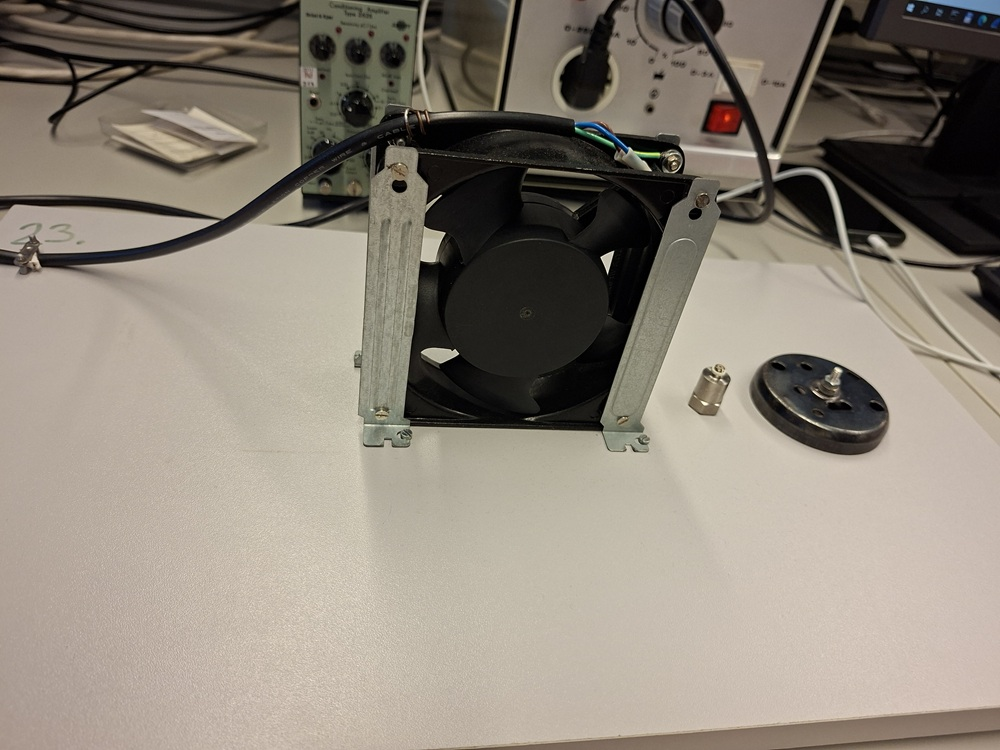
\includegraphics[width = \textwidth]{../../Kepek/20260914_142213.jpg}	
	\caption{A mérési elrendezés.}
	\label{fig:meresi-elrendezes}
\end{figure}

\subsubsection*{Feladat megoldása}
Első lépésben egy előre meghatározott frekvenciájú szinussz jel legenerálása volt a cél. A kezdeti fázist 0-nak választottuk, és minden időlépésben növeltük egy deltaPhase értékkel, amit az alábbi összefüggéssel határoztunk meg:

\begin{equation}
	deltaPhase = rbits\left(\dfrac{(outFreq<<15)}{sampleFreq} \mathbin{\&} mask\right)
\end{equation}

A kártya 48 kHz mintavételi frekvenciával rendelkezik, ezért a sampleFreq értékét 48000-ra állítottuk. A mask értéke pedig 32767 volt, hogy a 15 bites tartományon belül maradjunk.\\

Amikor a fázis értékének növelése után telítettük a fract értéktartományát, akkor kiszámítottuk mennyit kellene még növelnünk az aktuális fázis értéken, ahhoz hogy elérjük a \texttt{FRACT\_MAX}-ot, majd a 0-ról indulva a deltaPhase és ennek a remainingPhsae értékek a különbségére léptettük a fázist, ezzel megoldva azt, hogy ne legyen töréspontunk az egyes érték átlépése esetén.\\

A szinusz jelet a \texttt{sin2pi\_01\_fx16} függvény segítségével generáltuk, ami a fázis értékét használva adta vissza a megfelelő szinusz értéket. Az így kapott értéket a \texttt{process\_data} függvényben a iChannel0RightOut változóba mentettük, ami így már oszcilloszkópon is láthatóvá vált. \abrara{fig:szinuszjel} % kepet cserelni kell

\begin{figure}[H]
	\centering
	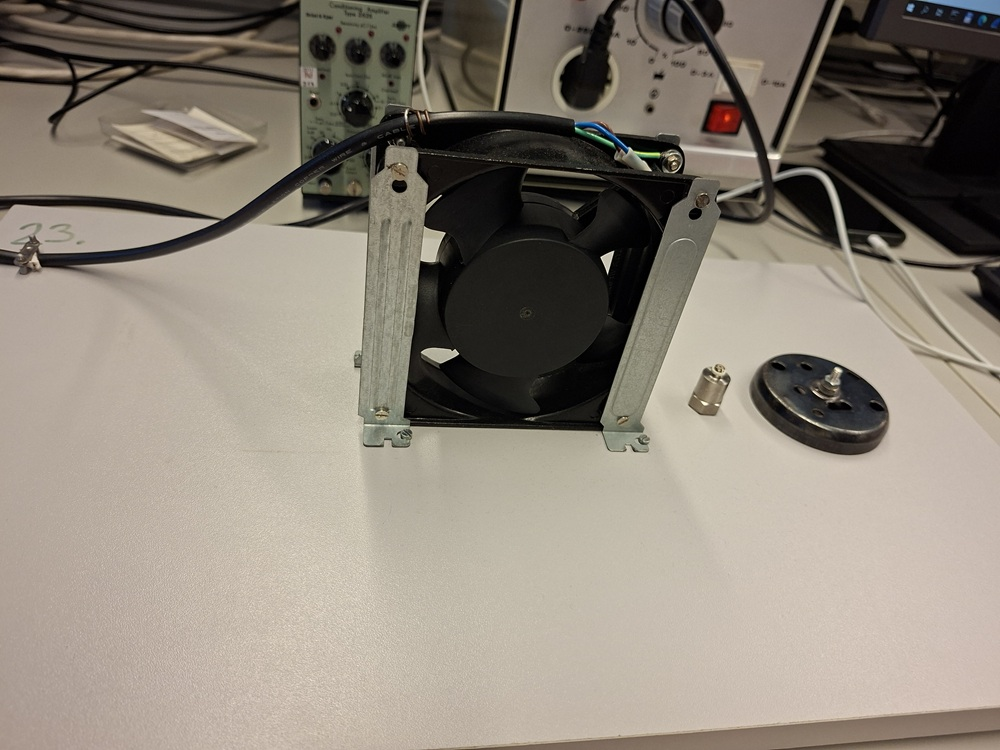
\includegraphics[width = \textwidth]{../../Kepek/20260914_142213.jpg}	
	\caption{A szinuszjel.}
	\label{fig:szinuszjel}
\end{figure}

\section*{Függelék}
\subsection*{Felhasznált C kódok}

\lstinputlisting[
    caption={process\_data.c},
    label={lst:process_data.c}
]{../../BlackFin_FIR_fract/src/process_data.c}

\lstinputlisting[
    caption={sin2pi\_fx.c},
    label={lst:sin2pi_fx.c}
]{../../BlackFin_FIR_fract/src/sin2pi_fx.c}

\lstinputlisting[
    caption={sin2pi\_fx.h},
    label={lst:sin2pi_fx.h}
]{../../BlackFin_FIR_fract/src/sin2pi_fx.h}

\end{document}
